%LTeX: language=it
\section{Casi d'uso}

    %LTeX: language=it
\subsection{UC 1 - Inviare un'e-mail} \label{sec:UC1}
    \begin{figure}[h]
        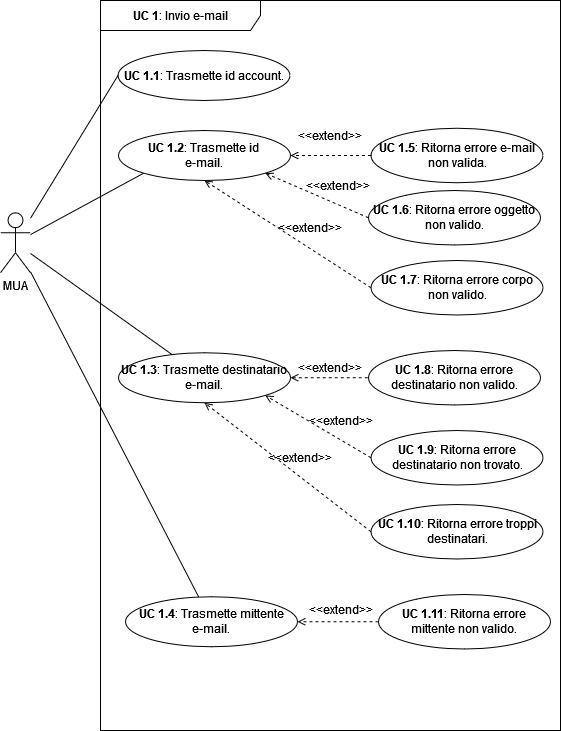
\includegraphics[width=0.85\textwidth]{sections/uc_imgs/UC01.png}
        \centering
        \caption{Diagramma UC 1.}
    \end{figure}
    \begin{itemize}
        \item \textbf{Attore principale}: MUA;
        \item \textbf{Descrizione}: il MUA deve poter inviare una e-mail al destinatario indicato;
        \item \textbf{Precondizioni}: l’account che il MUA gestisce è registrato nel sistema, e ha un connessione aperta con il sistema ed è autenticato;
        \item \textbf{Postcondizioni}: l'e-mail è stata consegnata con successo al destinatario, ed è stata salvata nel sistema;
        \item \textbf{Scenario principale}:
            \begin{enumerate}
                \item il MUA trasmette il destinatario dell'e-mail (\hyperref[sec:UC1.1]{UC 1.1});
                \item il MUA trasmette il mittente dell'e-mail (\hyperref[sec:UC1.2]{UC 1.2});
                \item il MUA trasmette l'oggetto dell'e-mail (\hyperref[sec:UC1.3]{UC 1.3});
                \item il MUA trasmette il corpo dell'e-mail (\hyperref[sec:UC1.4]{UC 1.4});
                \item il sistema salva l'e-mail nel mailbox;
                \item il sistema elabora l'inoltro;
            \end{enumerate}
        \item \textbf{Inclusioni}: nessuna;
        \item \textbf{Generalizzazioni}: nessuna;
        \item \textbf{Estensioni}: 
            \begin{enumerate}[label=\alph*.]
                \item il sistema incontra un errore durante il tentativo d'invio dell'e-mail:
                \begin{enumerate}[label=\arabic*.]
                    \item invia l'e-mail con il codice d'errore al MUA (\hyperref[sec:UC2]{UC 2}).
                \end{enumerate}
            \end{enumerate}
    \end{itemize}

    \begin{figure}[h]
        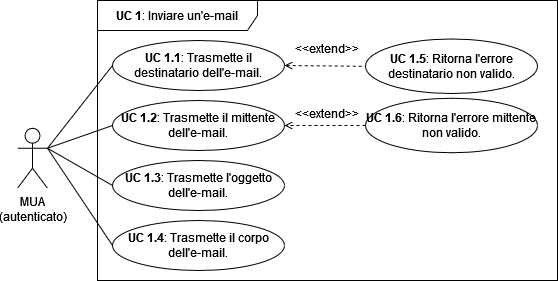
\includegraphics[width=0.75\textwidth]{sections/uc_imgs/UC01.X.png}
        \centering
        \caption{Diagramma sotto-casi UC 1.}
    \end{figure}

    \subsubsection{UC 1.1 - Trasmette il destinatario dell'e-mail} \label{sec:UC1.1}
    \begin{itemize}
        \item \textbf{Attore}: MUA;
        \item \textbf{Descrizione}: il MUA invia al sistema il destinatario dell'e-mail;
        \item \textbf{Precondizioni}: il MUA sta usando la funzionalità d'invio di un'e-mail;
        \item \textbf{Postcondizioni}: il sistema conosce l'indirizzo di posta elettronica del destinatario dell'e-mail;
        \item \textbf{Scenario principale}:
            \begin{enumerate}
                \item il MUA trasmette il destinatario, deve soddisfare il seguente requisito:
                    \begin{itemize}
                        \item l'indirizzo e-mail deve essere sintatticamente valido;
                    \end{itemize}
            \end{enumerate}
        \item \textbf{Inclusioni}: nessuna;
        \item \textbf{Generalizzazioni}: nessuna;
        \item \textbf{Estensioni}:
            \begin{enumerate}[label=\alph*.]
                \item l'indirizzo e-mail non è sintatticamente valido:
                \begin{enumerate}[label=\arabic*.]
                    \item il sistema invia un messaggio di errore al MUA (\hyperref[sec:UC1.6]{UC 1.6}).
                \end{enumerate}
            \end{enumerate}
    \end{itemize}

    \subsubsection{UC 1.2 - Trasmette il mittente dell'e-mail} \label{sec:UC1.2}
    \begin{itemize}
        \item \textbf{Attore}: MUA;
        \item \textbf{Descrizione}: il MUA invia al sistema il mittente dell'e-mail;
        \item \textbf{Precondizioni}: il MUA sta usando la funzionalità d'invio di un'e-mail;
        \item \textbf{Postcondizioni}: il sistema conosce l'indirizzo di posta elettronica del mittente dell'e-mail;
        \item \textbf{Scenario principale}:
            \begin{enumerate}
                \item il MUA trasmette il mittente, deve soddisfare il seguente requisito:
                    \begin{itemize}
                        \item l'indirizzo e-mail deve essere sintatticamente valido;
                    \end{itemize}
            \end{enumerate}
        \item \textbf{Inclusioni}: nessuna;
        \item \textbf{Generalizzazioni}: nessuna;
        \item \textbf{Estensioni}:
            \begin{enumerate}[label=\alph*.]
                \item l'indirizzo e-mail non è sintatticamente valido:
                \begin{enumerate}[label=\arabic*.]
                    \item il sistema invia un messaggio di errore al MUA (\hyperref[sec:UC1.7]{UC 1.7}).
                \end{enumerate}
            \end{enumerate}
    \end{itemize}

    \subsubsection{UC 1.3 - Trasmette l'oggetto dell'e-mail} \label{sec:UC1.3}
    \begin{itemize}
        \item \textbf{Attore}: MUA;
        \item \textbf{Descrizione}: il MUA invia al sistema l'oggetto dell'e-mail;
        \item \textbf{Precondizioni}: il MUA sta usando la funzionalità d'invio di un'e-mail;
        \item \textbf{Postcondizioni}: il sistema conosce l'oggetto dell'e-mail;
        \item \textbf{Scenario principale}:
            \begin{enumerate}
                \item il MUA trasmette l'oggetto dell'e-mail;
            \end{enumerate}
        \item \textbf{Inclusioni}: nessuna;
        \item \textbf{Generalizzazioni}: nessuna;
        \item \textbf{Estensioni}: nessuna.
    \end{itemize}

    \subsubsection{UC 1.4 - Trasmette il corpo dell'e-mail} \label{sec:UC1.4}
    \begin{itemize}
        \item \textbf{Attore}: MUA;
        \item \textbf{Descrizione}: il MUA invia al sistema il corpo dell'e-mail;
        \item \textbf{Precondizioni}: il MUA sta usando la funzionalità d'invio di un'e-mail;
        \item \textbf{Postcondizioni}: il sistema conosce il corpo dell'e-mail;
        \item \textbf{Scenario principale}:
            \begin{enumerate}
                \item il MUA trasmette il corpo dell'e-mail;
            \end{enumerate}
        \item \textbf{Inclusioni}: nessuna;
        \item \textbf{Generalizzazioni}: nessuna;
        \item \textbf{Estensioni}: nessuna.
    \end{itemize}



    \subsubsection{UC 1.5 - Ritorna l'errore destinatario non valido} \label{sec:UC1.5}
    \begin{itemize}
        \item \textbf{Attore}: MUA;
        \item \textbf{Descrizione}: il MUA riceve l'errore che il destinatario non è valido;
        \item \textbf{Precondizioni}: il MUA ha inviato il destinatario;
        \item \textbf{Postcondizioni}: il MUA viene notificato che il destinatario non è valido;
        \item \textbf{Scenario principale}:
            \begin{enumerate}
                \item il sistema controlla la sintassi del destinatario e trova un errore;
                \item il sistema notifica il MUA che il destinatario non è valido;
            \end{enumerate}
        \item \textbf{Inclusioni}: nessuna;
        \item \textbf{Generalizzazioni}: nessuna;
        \item \textbf{Estensioni}: nessuna.
    \end{itemize}

    \subsubsection{UC 1.6 - Ritorna l'errore mittente non valido} \label{sec:UC1.6}
    \begin{itemize}
        \item \textbf{Attore}: MUA;
        \item \textbf{Descrizione}: il MUA riceve l'errore che il mittente non è valido;
        \item \textbf{Precondizioni}: il MUA ha inviato il mittente;
        \item \textbf{Postcondizioni}: il MUA viene notificato che il mittente non è valido;
        \item \textbf{Scenario principale}:
            \begin{enumerate}
                \item il sistema controlla la sintassi del mittente e trova un errore;
                \item il sistema notifica il MUA che il mittente non è valido;
            \end{enumerate}
        \item \textbf{Inclusioni}: nessuna;
        \item \textbf{Generalizzazioni}: nessuna;
        \item \textbf{Estensioni}: nessuna.
    \end{itemize}



        % \subsubsection{UC 1.5 - Trasmettere gli allegati dell'e-mail} \label{sec:UC1.5}
    % \begin{itemize}
    %     \item \textbf{Attore}: MUA;
    %     \item \textbf{Descrizione}: il MUA invia al sistema il mittente dell'e-mail;
    %     \item \textbf{Precondizioni}: il MUA sta usando la funzionalità d'invio di un'e-mail;
    %     \item \textbf{Postcondizioni}: il sistema conosce l'indirizzo di posta elettronica del mittente dell'e-mail;
    %     \item \textbf{Scenario principale}:
    %         \begin{enumerate}
    %             \item il MUA trasmette gli allegati;
    %         \end{enumerate}
    %     \item \textbf{Inclusioni}: nessuna;
    %     \item \textbf{Generalizzazioni}: nessuna;
    %     \item \textbf{Estensioni}: 
    %         \begin{enumerate}[label=\alph*.]
    %             \item l'allegato supera la dimensione massima supporta dal sistema:
    %                 \begin{enumerate}[label=\arabic*.]
    %                     \item il sistema invia un messaggio di errore al MUA (\hyperref[sec:UC1.6]{UC 1.6}).
    %                 \end{enumerate}
    %         \end{enumerate}
    % \end{itemize}

    % \subsubsection{UC 1.8 - Ritorna l'errore massima dimensione allegati} \label{sec:UC1.8}
    % \begin{itemize}
    %     \item \textbf{Attore}: MUA;
    %     \item \textbf{Descrizione}: il MUA viene notificato che gli allegati dell'e-mail hanno superato la massima dimensione supportata;
    %     \item \textbf{Precondizioni}: il MUA sta usando di trasmissione degli allegati;
    %     \item \textbf{Postcondizioni}: il MUA è stato notificato del superamento della massima dimensione per gli allegati;
    %     \item \textbf{Scenario principale}:
    %         \begin{enumerate}
    %             \item il sistema controlla la dimensione degli allegati;
    %             \item il sistema nota che la dimensione è stata superata;
    %             \item il sistema notifica il MUA che la dimensione degli allegati supera la massima dimensione consentita per un e-mail;
    %         \end{enumerate}
    %     \item \textbf{Inclusioni}: nessuna;
    %     \item \textbf{Generalizzazioni}: nessuna;
    %     \item \textbf{Estensioni}: nessuna.
    % \end{itemize}
    
%LTeX: language=it
\subsection{UC 2 - Creare un'e-mail} \label{sec:UC2}
    \begin{figure}[h]
        %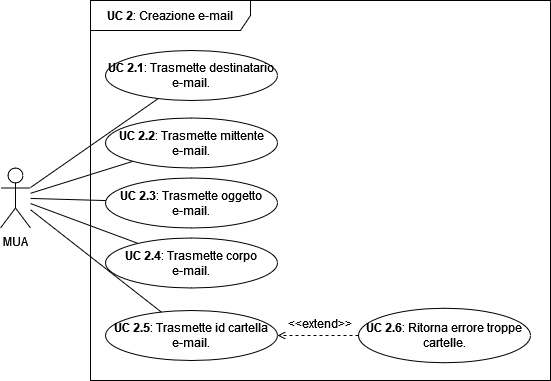
\includegraphics[width=0.85\textwidth]{sections/uc_imgs/UC02.png}
        \centering
        \caption{Diagramma UC 2.}
    \end{figure}
    \begin{itemize}
        \item \textbf{Attore principale}: MUA;
        \item \textbf{Descrizione}: il MUA deve poter inviare una e-mail al destinatario indicato;
        \item \textbf{Precondizioni}: l’account che il MUA gestisce è registrato nel sistema, e ha un connessione aperta con il sistema ed è autenticato;
        \item \textbf{Postcondizioni}: l'e-mail è stata consegnata con successo al destinatario, ed è stata salvata nel sistema;
        \item \textbf{Scenario principale}:
            \begin{enumerate}
                \item il MUA trasmette il destinatario dell'e-mail (\hyperref[sec:UC2.1]{UC 2.1});
                \item il MUA trasmette il mittente dell'e-mail (\hyperref[sec:UC2.2]{UC 2.2});
                \item il MUA trasmette l'oggetto dell'e-mail (\hyperref[sec:UC2.3]{UC 2.3});
                \item il MUA trasmette il corpo dell'e-mail (\hyperref[sec:UC2.4]{UC 2.4});
                \item il sistema salva l'e-mail nel mailbox;
                \item il sistema elabora l'inoltro;
            \end{enumerate}
        \item \textbf{Inclusioni}: nessuna;
        \item \textbf{Generalizzazioni}: nessuna;
        \item \textbf{Estensioni}: 
            \begin{enumerate}[label=\alph*.]
                \item il sistema incontra un errore durante il tentativo d'invio dell'e-mail:
                \begin{enumerate}[label=\arabic*.]
                    \item invia l'e-mail con il codice d'errore al MUA (\hyperref[sec:UC2]{UC 2}).
                \end{enumerate}
            \end{enumerate}
    \end{itemize}

    \begin{figure}[h]
        %\includegraphics[width=0.75\textwidth]{sections/uc_imgs/UC02.X.png}
        \centering
        \caption{Diagramma sotto-casi UC 2.}
    \end{figure}

    \subsubsection{UC 2.1 - Trasmette il destinatario dell'e-mail} \label{sec:UC2.1}
    \begin{itemize}
        \item \textbf{Attore}: MUA;
        \item \textbf{Descrizione}: il MUA invia al sistema il destinatario dell'e-mail;
        \item \textbf{Precondizioni}: il MUA sta usando la funzionalità d'invio di un'e-mail;
        \item \textbf{Postcondizioni}: il sistema conosce l'indirizzo di posta elettronica del destinatario dell'e-mail;
        \item \textbf{Scenario principale}:
            \begin{enumerate}
                \item il MUA trasmette il destinatario, deve soddisfare il seguente requisito:
                    \begin{itemize}
                        \item l'indirizzo e-mail deve essere sintatticamente valido;
                    \end{itemize}
            \end{enumerate}
        \item \textbf{Inclusioni}: nessuna;
        \item \textbf{Generalizzazioni}: nessuna;
        \item \textbf{Estensioni}:
            \begin{enumerate}[label=\alph*.]
                \item l'indirizzo e-mail non è sintatticamente valido:
                \begin{enumerate}[label=\arabic*.]
                    \item il sistema invia un messaggio di errore al MUA (\hyperref[sec:UC2.6]{UC 2.6}).
                \end{enumerate}
            \end{enumerate}
    \end{itemize}

    \subsubsection{UC 2.2 - Trasmette il mittente dell'e-mail} \label{sec:UC2.2}
    \begin{itemize}
        \item \textbf{Attore}: MUA;
        \item \textbf{Descrizione}: il MUA invia al sistema il mittente dell'e-mail;
        \item \textbf{Precondizioni}: il MUA sta usando la funzionalità d'invio di un'e-mail;
        \item \textbf{Postcondizioni}: il sistema conosce l'indirizzo di posta elettronica del mittente dell'e-mail;
        \item \textbf{Scenario principale}:
            \begin{enumerate}
                \item il MUA trasmette il mittente, deve soddisfare il seguente requisito:
                    \begin{itemize}
                        \item l'indirizzo e-mail deve essere sintatticamente valido;
                    \end{itemize}
            \end{enumerate}
        \item \textbf{Inclusioni}: nessuna;
        \item \textbf{Generalizzazioni}: nessuna;
        \item \textbf{Estensioni}:
            \begin{enumerate}[label=\alph*.]
                \item l'indirizzo e-mail non è sintatticamente valido:
                \begin{enumerate}[label=\arabic*.]
                    \item il sistema invia un messaggio di errore al MUA (\hyperref[sec:UC2.7]{UC 2.7}).
                \end{enumerate}
            \end{enumerate}
    \end{itemize}

    \subsubsection{UC 2.3 - Trasmette l'oggetto dell'e-mail} \label{sec:UC2.3}
    \begin{itemize}
        \item \textbf{Attore}: MUA;
        \item \textbf{Descrizione}: il MUA invia al sistema l'oggetto dell'e-mail;
        \item \textbf{Precondizioni}: il MUA sta usando la funzionalità d'invio di un'e-mail;
        \item \textbf{Postcondizioni}: il sistema conosce l'oggetto dell'e-mail;
        \item \textbf{Scenario principale}:
            \begin{enumerate}
                \item il MUA trasmette l'oggetto dell'e-mail;
            \end{enumerate}
        \item \textbf{Inclusioni}: nessuna;
        \item \textbf{Generalizzazioni}: nessuna;
        \item \textbf{Estensioni}: nessuna.
    \end{itemize}

    \subsubsection{UC 2.4 - Trasmette il corpo dell'e-mail} \label{sec:UC2.4}
    \begin{itemize}
        \item \textbf{Attore}: MUA;
        \item \textbf{Descrizione}: il MUA invia al sistema il corpo dell'e-mail;
        \item \textbf{Precondizioni}: il MUA sta usando la funzionalità d'invio di un'e-mail;
        \item \textbf{Postcondizioni}: il sistema conosce il corpo dell'e-mail;
        \item \textbf{Scenario principale}:
            \begin{enumerate}
                \item il MUA trasmette il corpo dell'e-mail;
            \end{enumerate}
        \item \textbf{Inclusioni}: nessuna;
        \item \textbf{Generalizzazioni}: nessuna;
        \item \textbf{Estensioni}: nessuna.
    \end{itemize}



    \subsubsection{UC 2.5 - Ritorna l'errore destinatario non valido} \label{sec:UC2.5}
    \begin{itemize}
        \item \textbf{Attore}: MUA;
        \item \textbf{Descrizione}: il MUA riceve l'errore che il destinatario non è valido;
        \item \textbf{Precondizioni}: il MUA ha inviato il destinatario;
        \item \textbf{Postcondizioni}: il MUA viene notificato che il destinatario non è valido;
        \item \textbf{Scenario principale}:
            \begin{enumerate}
                \item il sistema controlla la sintassi del destinatario e trova un errore;
                \item il sistema notifica il MUA che il destinatario non è valido;
            \end{enumerate}
        \item \textbf{Inclusioni}: nessuna;
        \item \textbf{Generalizzazioni}: nessuna;
        \item \textbf{Estensioni}: nessuna.
    \end{itemize}

    \subsubsection{UC 2.6 - Ritorna l'errore mittente non valido} \label{sec:UC2.6}
    \begin{itemize}
        \item \textbf{Attore}: MUA;
        \item \textbf{Descrizione}: il MUA riceve l'errore che il mittente non è valido;
        \item \textbf{Precondizioni}: il MUA ha inviato il mittente;
        \item \textbf{Postcondizioni}: il MUA viene notificato che il mittente non è valido;
        \item \textbf{Scenario principale}:
            \begin{enumerate}
                \item il sistema controlla la sintassi del mittente e trova un errore;
                \item il sistema notifica il MUA che il mittente non è valido;
            \end{enumerate}
        \item \textbf{Inclusioni}: nessuna;
        \item \textbf{Generalizzazioni}: nessuna;
        \item \textbf{Estensioni}: nessuna.
    \end{itemize}

    %LTeX: language=it
\subsection{UC 3 - Creazione cartella} \label{sec:UC3}
    \begin{itemize}
        \item \textbf{Attore principale}: MUA;
        \item \textbf{Descrizione}: il MUA deve poter creare una cartella nel sistema;
        \item \textbf{Precondizioni}: l’account che il MUA gestisce è registrato nel sistema, e ha una connessione aperta con il sistema ed è autenticato;
        \item \textbf{Postcondizioni}: il MUA crea la cartella che viene salvata nel sistema;
        \item \textbf{Scenario principale}:
            \begin{enumerate}
                \item il MUA trasmette il nome della cartella (\hyperref[sec:UC3.1]{UC 3.1});
                \item il MUA trasmette l'id della cartella genitore (\hyperref[sec:UC3.2]{UC 3.2});
                \item il sistema salva la nuova cartella.
            \end{enumerate}
        \item \textbf{Inclusioni}: nessuna;
        \item \textbf{Generalizzazioni}: nessuna;
        \item \textbf{Estensioni}: nessuna.
    \end{itemize}

\begin{figure}[H]
    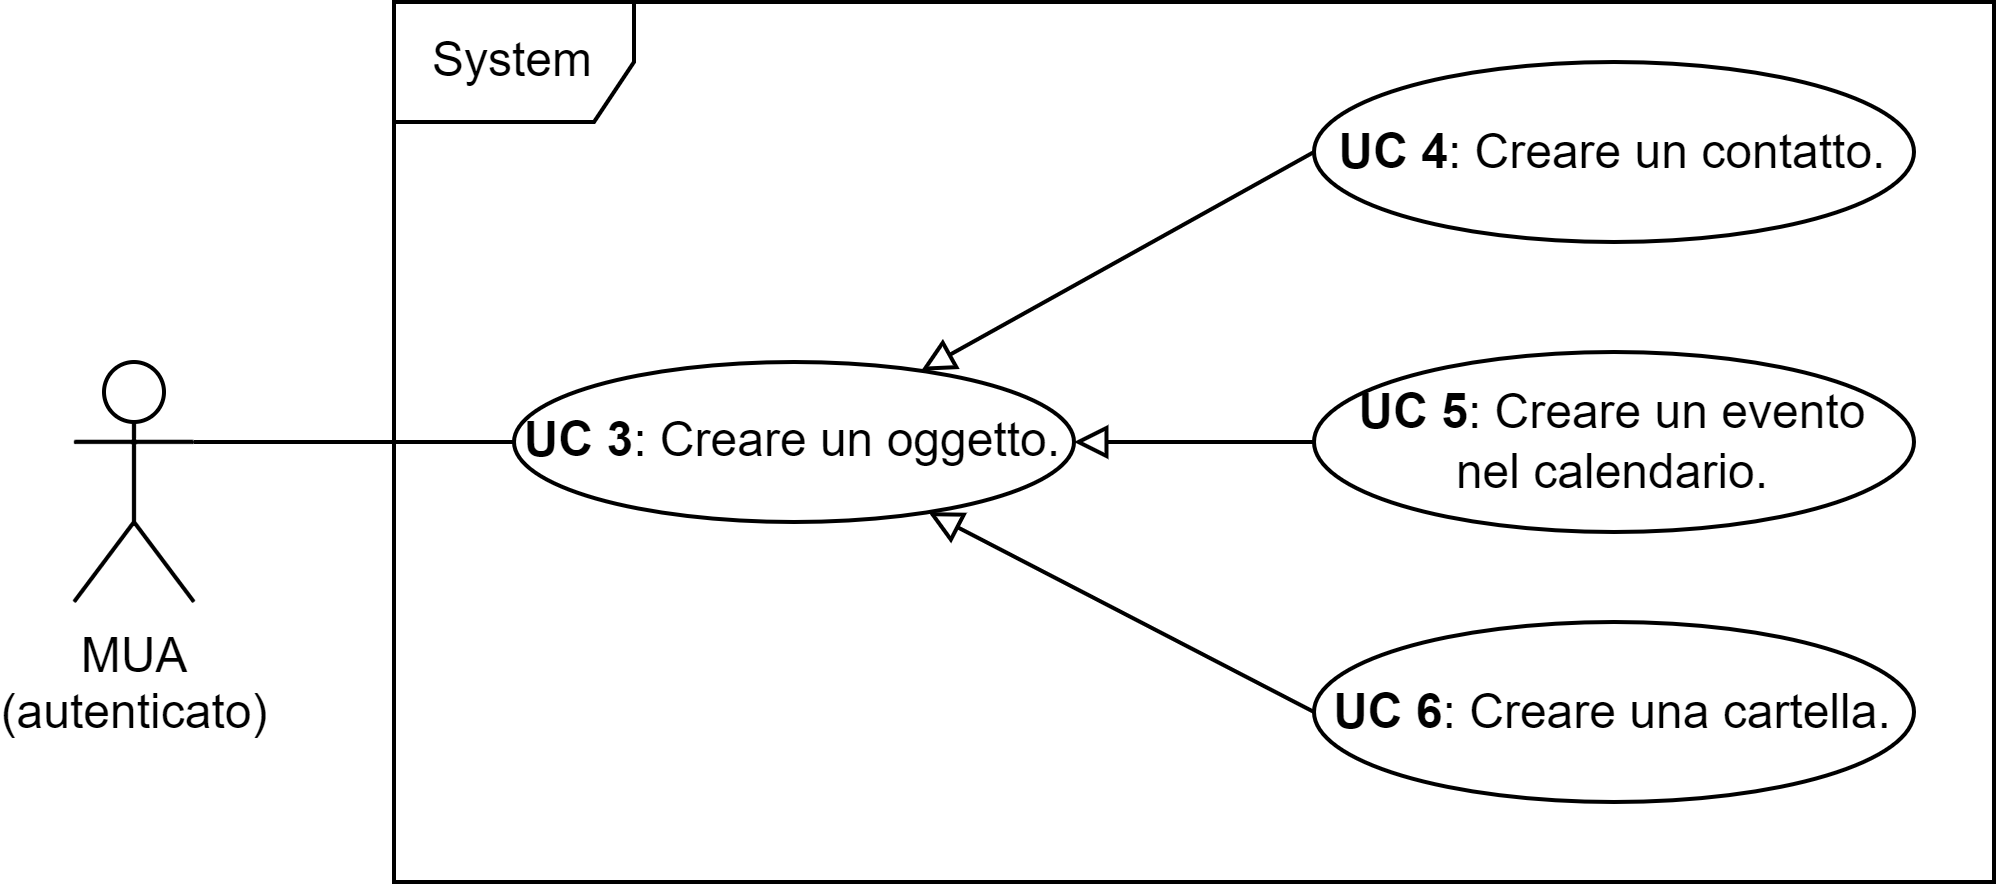
\includegraphics[width=0.85\textwidth]{sections/uc_imgs/UC03.png}
    \centering
    \caption{Diagramma sotto-casi UC 3}
\end{figure}

\subsubsection{UC 3.1 - Trasmette nome cartella} \label{sec:UC3.1}
    \begin{itemize}
        \item \textbf{Attore principale}: MUA;
        \item \textbf{Descrizione}: il MUA trasmette il nome per creare la cartella al sistema;
        \item \textbf{Precondizioni}: il MUA sta usando la funzionalità di creazione di una cartella;
        \item \textbf{Postcondizioni}: il sistema conosce il nome della cartella;
        \item \textbf{Scenario principale}:
            \begin{enumerate}
                \item il MUA invia il nome per creare la cartella al sistema;
                \item il sistema controlla che le informazioni ricevute rispettino il seguente requisito minimo:
                \begin{itemize}
                    \item il nome ricevuto non è una stringa vuota.
                \end{itemize}
            \end{enumerate}
        \item \textbf{Inclusioni}: nessuna;
        \item \textbf{Generalizzazioni}: nessuna;
        \item \textbf{Estensioni}:
            \begin{enumerate}[label=\alph*.]
                \item il sistema non riesce a creare la cartella perché il nome fornito non è valido:
                \begin{enumerate}[label=\arabic*.]
                    \item il sistema ritorna un errore al MUA di nome non valido (\hyperref[sec:UC3.3]{UC 3.3}).
                \end{enumerate}
            \end{enumerate}
    \end{itemize}

    \subsubsection{UC 3.2 - Trasmette id cartella genitore} \label{sec:UC3.2}
    \begin{itemize}
        \item \textbf{Attore principale}: MUA;
        \item \textbf{Descrizione}: il MUA trasmette l'id della cartella genitore al sistema;
        \item \textbf{Precondizioni}: il MUA sta usando la funzionalità di creazione di una cartella;
        \item \textbf{Postcondizioni}: il sistema conosce l'id della cartella genitore;
        \item \textbf{Scenario principale}:
            \begin{enumerate}
                \item il MUA invia le informazioni necessarie per creare la cartella;
                \item il sistema elabora le informazioni ricevute, controlla che:
                \begin{itemize}
                    \item la cartella genitore esista.
                \end{itemize}
            \end{enumerate}
        \item \textbf{Inclusioni}: nessuna;
        \item \textbf{Generalizzazioni}: nessuna;
        \item \textbf{Estensioni}:
            \begin{enumerate}[label=\alph*.]
                \item il sistema non riesce a salvare la cartella perché non trova la cartella genitore:
                \begin{enumerate}[label=\arabic*.]
                    \item il sistema ritorna un errore al MUA di cartella genitore non trovata (\hyperref[sec:UC3.4]{UC 3.4});
                    \end{enumerate}
                \item il sistema non riesce a salvare la cartella perché è un duplicato:
                \begin{enumerate}[label=\arabic*.]
                    \item il sistema ritorna un errore al MUA di cartella duplicata (\hyperref[sec:UC3.5]{UC 3.5}).
                \end{enumerate}
                
            \end{enumerate}
    \end{itemize}



    \subsubsection{UC 3.3 - Ritorna errore nome non valido} \label{sec:UC3.3}
    \begin{itemize}
        \item \textbf{Attore principale}: MUA;
        \item \textbf{Descrizione}: il MUA riceve l'errore che il nome della cartella non è valido;
        \item \textbf{Precondizioni}:  il MUA ha trasmesso il nome per creare la cartella al sistema;
        \item \textbf{Postcondizioni}: il sistema non crea la nuova cartella e il MUA viene notificato dell'errore;
        \item \textbf{Scenario principale}:
            \begin{enumerate}
                \item il sistema controlla la sintassi del nome e trova un errore;
                \item il sistema non crea la cartella e notifica il MUA dell'errore.
            \end{enumerate}
        \item \textbf{Inclusioni}: nessuna;
        \item \textbf{Generalizzazioni}: nessuna;
        \item \textbf{Estensioni}: nessuna.
    \end{itemize}

    \subsubsection{UC 3.4 - Ritorna errore cartella genitore non trovata} \label{sec:UC3.4}
    \begin{itemize}
        \item \textbf{Attore principale}: MUA;
        \item \textbf{Descrizione}: il MUA riceve l'errore che la cartella genitore non è stata trovata;
        \item \textbf{Precondizioni}: il MUA ha trasmesso l'id della cartella genitore al sistema;
        \item \textbf{Postcondizioni}: il sistema non crea la nuova cartella e il MUA viene notificato dell'errore;
        \item \textbf{Scenario principale}:
            \begin{enumerate}
                \item il sistema non trova l'di fornito;
                \item il sistema non crea la cartella e notifica il MUA dell'errore.
            \end{enumerate}
        \item \textbf{Inclusioni}: nessuna;
        \item \textbf{Generalizzazioni}: nessuna;
        \item \textbf{Estensioni}: nessuna.
    \end{itemize}

\subsubsection{UC 3.5 - Ritorna errore cartella duplicata} \label{sec:UC3.5}
    \begin{itemize}
        \item \textbf{Attore principale}: MUA;
        \item \textbf{Descrizione}: il MUA riceve l'errore che la cartella è duplicata;
        \item \textbf{Precondizioni}: il MUA ha trasmesso i dettagli per creare la cartella al sistema;
        \item \textbf{Postcondizioni}: il sistema non crea la nuova cartella e il MUA viene notificato dell'errore;
        \item \textbf{Scenario principale}:
            \begin{enumerate}
                \item il sistema nota che la cartella esiste già e annulla l'operazione per la creazione della cartella;
                \item il sistema non crea la cartella e notifica il MUA dell'errore.
            \end{enumerate}
        \item \textbf{Inclusioni}: nessuna;
        \item \textbf{Generalizzazioni}: nessuna;
        \item \textbf{Estensioni}: nessuna.
    \end{itemize}


    %LTeX: language=it
\subsection{UC 4 - Creazione contatto} \label{sec:UC4}
    \begin{itemize}
        \item \textbf{Attore principale}: MUA;
        \item \textbf{Descrizione}: il MUA deve poter creare un contatto nel sistema;
        \item \textbf{Precondizioni}: l’account che il MUA gestisce è registrato nel sistema, ha una connessione aperta con il sistema ed è autenticato;
        \item \textbf{Postcondizioni}: il MUA crea il contatto che viene salvato nel sistema;
        \item \textbf{Scenario principale}:
            \begin{enumerate}
                \item il MUA trasmette il nome del contatto (\hyperref[sec:UC4.1]{UC 4.1});
                \item il MUA trasmette l'indirizzo e-mail del contatto (\hyperref[sec:UC4.2]{UC 4.2});
                \item il sistema salva il contatto;
            \end{enumerate}
        \item \textbf{Inclusioni}: nessuna;
        \item \textbf{Generalizzazioni}: nessuna;
        \item \textbf{Estensioni}: nessuna.
    \end{itemize}

\begin{figure}[H]
    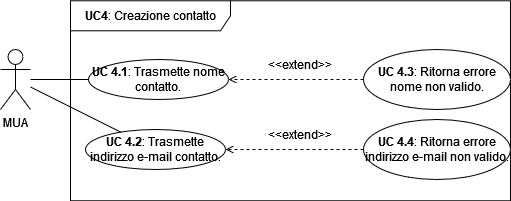
\includegraphics[width=0.85\textwidth]{sections/uc_imgs/UC04.png}
    \centering
    \caption{Diagramma sotto-casi UC 4}
\end{figure}

\subsubsection{UC 4.1 - Trasmette nome contatto} \label{sec:UC4.1}
    \begin{itemize}
        \item \textbf{Attore principale}: MUA;
        \item \textbf{Descrizione}: il MUA trasmette il nome per creare il contatto al sistema;
        \item \textbf{Precondizioni}: il MUA sta usando la funzionalità di creazione di un contatto;
        \item \textbf{Postcondizioni}: il sistema conosce il nome del contatto;
        \item \textbf{Scenario principale}:
            \begin{enumerate}
                \item il MUA invia il nome per creare il contatto al sistema;
                \item il sistema controlla che le informazioni ricevute rispettino il seguente requisito minimo:
                    \begin{itemize}
                        \item il nome del contatto non è una stringa vuota;
                    \end{itemize}
            \end{enumerate}
        \item \textbf{Inclusioni}: nessuna;
        \item \textbf{Generalizzazioni}: nessuna;
        \item \textbf{Estensioni}:
            \begin{enumerate}[label=\alph*.]
                \item il sistema non riesce a creare il contatto perché il nome fornito non è valido:
                \begin{enumerate}[label=\arabic*.]
                    \item il sistema ritorna un errore al MUA di nome non valido (\hyperref[sec:UC4.3]{UC 4.3}).
                \end{enumerate}
            \end{enumerate}
    \end{itemize}


    \subsubsection{UC 4.2 - Trasmette indirizzo e-mail contatto} \label{sec:UC4.2}
    \begin{itemize}
        \item \textbf{Attore principale}: MUA;
        \item \textbf{Descrizione}: il MUA trasmette l'indirizzo e-mail per creare il contatto al sistema;
        \item \textbf{Precondizioni}: il MUA sta usando la funzionalità di creazione di un contatto;
        \item \textbf{Postcondizioni}: il sistema conosce l'indirizzo e-mail del contatto;
        \item \textbf{Scenario principale}:
            \begin{enumerate}
                \item il MUA invia l'indirizzo e-mail per creare il contatto al sistema;
                \item il sistema controlla che le informazioni ricevute rispettino il seguente requisito minimo:
                    \begin{itemize}
                        \item l'indirizzo e-mail del contatto non è una stringa vuota;
                    \end{itemize}
            \end{enumerate}
        \item \textbf{Inclusioni}: nessuna;
        \item \textbf{Generalizzazioni}: nessuna;
        \item \textbf{Estensioni}:
            \begin{enumerate}[label=\alph*.]
                \item il sistema non riesce a creare il contatto perché l'indirizzo e-mail fornito non è valido:
                \begin{enumerate}[label=\arabic*.]
                    \item il sistema ritorna un errore al MUA di indirizzo e-mail non valido (\hyperref[sec:UC4.4]{UC 4.4}).
                \end{enumerate}
            \end{enumerate}
    \end{itemize}




\subsubsection{UC 4.3 - Ritorna errore nome non valido} \label{sec:UC4.3}
    \begin{itemize}
        \item \textbf{Attore principale}: MUA;
        \item \textbf{Descrizione}: il sistema non riesce a salvare il contatto perché il nome del contatto non rispetta i requisiti;
        \item \textbf{Precondizioni}: il MUA ha inviato il nome del contatto;
        \item \textbf{Postcondizioni}: il sistema non salva il nuovo contatto, il MUA è stato notificato dell'errore;
        \item \textbf{Scenario principale}:
            \begin{enumerate}
                \item il sistema controlla la sintassi del nome del contatto e trova un errore;
                \item il sistema non salva il contatto e notifica il MUA dell'errore;
            \end{enumerate}
        \item \textbf{Inclusioni}: nessuna;
        \item \textbf{Generalizzazioni}: nessuna;
        \item \textbf{Estensioni}: nessuna.
    \end{itemize}

\subsubsection{UC 4.4 - Ritorna errore indirizzo e-mail non valido} \label{sec:UC4.4}
    \begin{itemize}
        \item \textbf{Attore principale}: MUA;
        \item \textbf{Descrizione}: il sistema non riesce a salvare il contatto perché l'indirizzo e-mail del contatto non rispetta i requisiti;
        \item \textbf{Precondizioni}: il MUA ha inviato l'indirizzo e-mail del contatto;
        \item \textbf{Postcondizioni}: il sistema non salva il nuovo contatto, il MUA è stato notificato dell'errore;
        \item \textbf{Scenario principale}:
            \begin{enumerate}
                \item il sistema controlla la sintassi dell'indirizzo e-mail del contatto e trova un errore;
                \item il sistema non salva il contatto e notifica il MUA dell'errore;
            \end{enumerate}
        \item \textbf{Inclusioni}: nessuna;
        \item \textbf{Generalizzazioni}: nessuna;
        \item \textbf{Estensioni}: nessuna.
    \end{itemize}

%     \subsubsection{UC 2.1 - Trasmettere richiesta di aggiornamento} \label{sec: UC 2.1}
%     \begin{itemize}
%         \item Attore: MUA;
%         \item Descrizione: il MUA deve poter richiedere un aggiornamento dei propri dati;
%         \item Scenario:
%         \begin{enumerate}
%         \item il MUA si connette con il server;
%         \item il MUA richiede nuovi dati.
%         \end{enumerate}
%         \item Estensioni: errore... %(\hyperref[sec: UC 1.4.1]{UC 1.4.1});
%         \item Precondizioni: il MUA si sta aggiornando con i nuovi dati;
%         \item Postcondizioni: il MUA ha ricevuto nuove informazioni.
%     \end{itemize}



%     \subsubsection{UC 3.1 - Creare una cartella} \label{sec: UC 3.1}
%     \begin{itemize}
%         \item Attore: MUA;
%         \item Descrizione: il MUA deve poter creare una cartella;
%         \item Scenario:
%             \begin{enumerate}
%             \item il MUA si connette con il server;
%             \item il MUA trasmette i dati necessari per creare la cartella; 
%             \item % scrivere trasmettere solo nome forse???
%             \end{enumerate}
%         \item Estensioni: Errore nome cartella
%         \item Precondizioni: il MUA sta creando una cartella;
%         \item Postcondizioni: è stata creata la cartella.
%     \end{itemize}

%     \subsubsection{UC 3.2 - Creare un contatto} \label{sec: UC 3.2}
%     \begin{itemize}
%         \item Attore: MUA;
%         \item Descrizione: il MUA deve poter creare un contatto;
%         \item Scenario:
%         \begin{enumerate}
%         \item il MUA si connette con il server;
%         \item il MUA trasmette i dati necessari per creare il contatto;
%         \end{enumerate}
%         \item Estensioni: errore...
%         \item Precondizioni: il MUA sta creando un contatto;
%         \item Postcondizioni: è stata creata il contatto.
%     \end{itemize}

%     \subsubsection{UC 3.3 - Creare una condivisione} \label{sec: UC 3.3}
%     \begin{itemize}
%         \item Attore: MUA;
%         \item Descrizione: il MUA deve poter creare una condivisione di una cartella;
%         \item Scenario:
%         \begin{enumerate}
%         \item il MUA si connette con il server;
%         \item il MUA trasmette i dati necessari per creare la condivisione della cartella.
%         \end{enumerate}
%         \item Estensioni: errore...
%         \item Precondizioni: l’account che il MUA gestisce è registrato nel sistema ed è autenticato;
%         \item Postcondizioni: è stata creata la condivisione di una cartella.
%     \end{itemize}

%     \subsubsection{UC 3.4 - Creare un evento} \label{sec: UC 3.4}
%     \begin{itemize}
%         \item Attore: MUA;
%         \item Descrizione: il MUA deve poter creare un evento;
%         \item Scenario:
%         \begin{enumerate}
%         \item il MUA si connette con il server;
%         \item il MUA trasmette i dati necessari per creare un evento.
%         \end{enumerate}
%         \item Estensioni: errore...
%         \item Precondizioni: il MUA sta creando un evento;
%         \item Postcondizioni: è stato creato l'evento.
%     \end{itemize}

%     \subsection{UC 4 - Modificare un oggetto} \label{sec: UC 4}
%     \begin{itemize}
%         \item Attore: MUA;
%         \item Descrizione: il MUA deve poter modificare un oggetto specifico;
%         \item Scenario principale:
%             \begin{enumerate}
%                 \item 
%             \end{enumerate}
%         \item Generalizzazioni:
%             \begin{itemize}
%             \item il MUA modifica una cartella (\hyperref[sec: UC 4.1]{UC 4.1});
%             \item il MUA modifica un contatto (\hyperref[sec: UC 4.2]{UC 4.2});
%             \item il MUA mofidica una condivisione (\hyperref[sec: UC 4.3]{UC 4.3});
%             \item il MUA modifica un evento (\hyperref[sec: UC 4.4]{UC 4.4}).
%             \end{itemize}
%         \item Estensioni: errore...
%         \item Precondizioni: l’account che il MUA gestisce è registrato nel sistema ed è autenticato;
%         \item Postcondizioni: è stato modificato l’oggetto desiderato.
%     \end{itemize}

%     \subsubsection{UC 4.1 - Modificare una cartella} \label{sec: UC 4.1}
%     \begin{itemize}
%         \item Attore: MUA;
%         \item Descrizione: il MUA deve poter modificare una cartella;
%         \item Scenario:
%         \begin{enumerate}
%         \item il MUA si connette con il server;
%         \item Il MUA trasmette i dati necessari per modificare la cartella.
%         \end{enumerate}
%         \item Estensioni: errore...
%         \item Precondizioni: il MUA sta modificando una cartella;
%         \item Postcondizioni: è stata modificata la cartella.
%     \end{itemize}

%     \subsubsection{UC 4.2 - Modificare un contatto} \label{sec: UC 4.2}
%     \begin{itemize}
%         \item Attore: MUA;
%         \item Descrizione: il MUA deve poter modificare un contatto;
%         \item Scenario:
%         \begin{enumerate}
%         \item il MUA si connette con il server;
%         \item Il MUA trasmette i dati necessari per modificare il contatto.
%         \end{enumerate}
%         \item Estensioni: errore...
%         \item Precondizioni: il MUA sta modificando un contatto;
%         \item Postcondizioni: è stato modificato il contatto.
%     \end{itemize}

%     \subsubsection{UC 4.3 - Modificare una condivisione} \label{sec: UC 4.3}
%     \begin{itemize}
%         \item Attore: MUA;
%         \item Descrizione: il MUA deve poter modificare una condivisione di una cartella;
%         \item Scenario:
%         \begin{enumerate}
%         \item il MUA si connette con il server;
%         \item Il MUA trasmette i dati necessari per modificare la condivisione di una cartella.
%         \end{enumerate}
%         \item Estensioni: errore...
%         \item Precondizioni: il MUA sta modificando una condivisione di una cartella;
%         \item Postcondizioni: è stata modificata la condivisione di una cartella.
%     \end{itemize}

%     \subsubsection{UC 4.4 - Modificare un evento} \label{sec: UC 4.4}
%     \begin{itemize}
%         \item Attore: MUA;
%         \item Descrizione: il MUA deve poter modificare un evento;
%         \item Scenario:
%         \begin{enumerate}
%         \item il MUA si connette con il server;
%         \item Il MUA trasmette i dati necessari per modificare un evento.
%         \end{enumerate}
%         \item Estensioni: 
%         \begin{itemize}
%             \item Errore dimensioni evento;
%         \end{itemize}
%         \item Precondizioni: il MUA sta modificando un evento;
%         \item Postcondizioni: è stato modificato l'evento.
%     \end{itemize}

%     \subsection{UC 5 - Eliminare un oggetto} \label{sec: UC 5}
%     \begin{itemize}
%         \item Attore: MUA;
%         \item Descrizione: il MUA deve poter eliminare un oggetto specifico;
%         \item Scenario principale:
%         \begin{enumerate}
%             \item 
%         \end{enumerate}
%         \item Generalizzazioni:
%             \begin{itemize}
%             \item il MUA elimina una cartella (\hyperref[sec: UC 5.1]{UC 5.1});
%             \item il MUA elimina un contatto (\hyperref[sec: UC 5.2]{UC 5.2});
%             \item il MUA elimina una condivisione (\hyperref[sec: UC 5.3]{UC 5.3});
%             \item il MUA elimina un evento (\hyperref[sec: UC 5.4]{UC 5.4}).
%             \end{itemize}
%         \item Estensioni:
%         \item Precondizioni: l’account che il MUA gestisce è registrato nel sistema ed è autenticato;
%         \item Postcondizioni: è stato eliminato l’oggetto desiderato.
%     \end{itemize}

%     \subsubsection{UC 5.1 - Eliminare una cartella} \label{sec: UC 5.1}
%     \begin{itemize}
%         \item Attore: MUA;
%         \item Descrizione: il MUA deve poter eliminare una cartella;
%         \item Scenario:
%         \begin{enumerate}
%         \item il MUA si connette con il server;
%         \item Il MUA trasmette i dati necessari per eliminare la cartella.
%         \end{enumerate}
%         \item Estensioni: 
%             \begin{itemize}
%                 \item Errore cartella contenente email;
%                 \item Errore cartella contenente cartelle;
%             \end{itemize}
%         \item Precondizioni: il MUA sta eliminando una cartella;
%         \item Postcondizioni: è stata eliminata la cartella.
%     \end{itemize}

%     \subsubsection{UC 5.2 - Eliminare un contatto} \label{sec: UC 5.2}
%     \begin{itemize}
%         \item Attore: MUA;
%         \item Descrizione: il MUA deve poter eliminare un contatto;
%         \item Scenario:
%         \begin{enumerate}
%         \item il MUA si connette con il server;
%         \item Il MUA trasmette i dati necessari per eliminare il contatto.
%         \end{enumerate}
%         \item Estensioni: errore...
%         \item Precondizioni: il MUA sta eliminando un contatto;
%         \item Postcondizioni: è stato eliminato il contatto.
%     \end{itemize}

%     \subsubsection{UC 5.3 - Eliminare una condivisione} \label{sec: UC 5.3}
%     \begin{itemize}
%         \item Attore: MUA;
%         \item Descrizione: il MUA deve poter eliminare una condivisione di una cartella;
%         \item Scenario:
%         \begin{enumerate}
%         \item il MUA si connette con il server;
%         \item Il MUA trasmette i dati necessari per eliminare la condivisione di una cartella.
%         \end{enumerate}
%         \item Estensioni: errore...
%         \item Precondizioni: il MUA sta eliminando una condivisione di una cartella;
%         \item Postcondizioni: è stata eliminata la condivisione di una cartella.
%     \end{itemize}

%     \subsubsection{UC 5.4 - Eliminare un evento} \label{sec: UC 5.4}
%     \begin{itemize}
%         \item Attore: MUA;
%         \item Descrizione: il MUA deve poter eliminare un evento;
%         \item Scenario:
%         \begin{enumerate}
%         \item il MUA si connette con il server;
%         \item Il MUA trasmette i dati necessari per eliminare un evento.
%         \end{enumerate}
%         \item Estensioni: errore...
%         \item Precondizioni: il MUA sta eliminando un evento;
%         \item Postcondizioni: è stato eliminato l'evento.
%     \end{itemize}


%     %creazione cartella problema nome
%     \paragraph{UC Errore nome cartella} \label{sec: UC 11.4.2.1}
%     \begin{itemize}
%         \item Attore: MUA;
%         \item Descrizione: il MUA deve ricevere un messaggio di errore adeguato quando si tenta la creazione di una cartella con lo stesso nome e la stessa cartella padre di un'altra;
%         \item Scenario:
%         \begin{enumerate}
%         \item il MUA riceve il messaggio di errore;
%         \end{enumerate}   
%         \item Precondizioni: 
%         \begin{enumerate}
%             \item il MUA ha trasmesso il nome per la creazione della cartella;
%             \item esiste già una cartella con lo stesso nome e la stessa cartella padre;
%         \end{enumerate}
%         \item Postcondizioni: il MUA ha ricevuto un messaggio di errore.
%     \end{itemize}

%     %modificare una cartella (tho anche per creare c'è)
%     \paragraph{UC Errore dimensioni cartella} \label{sec: UC 11.4.2.1}
%     \begin{itemize}
%         \item Attore: MUA;
%         \item Descrizione: il MUA deve ricevere un messaggio di errore adeguato quando la modifica di una o più caratteristiche di una cartella superano i limiti di dimensione stabiliti;
%         \item Scenario:
%         \begin{enumerate}
%         \item il MUA riceve il messaggio di errore;
%         \end{enumerate}   
%         \item Precondizioni: 
%         \begin{enumerate}
%             \item il MUA ha trasmesso i dati per la modifica di una cartella;
%             \item una o più caratteristiche di una cartella superano i limiti di dimensione stabiliti;
%         \end{enumerate}
%         \item Postcondizioni: il MUA ha ricevuto un messaggio di errore.
%     \end{itemize}

%     %modificare una cartella (tho anche per creare c'è)
%     \paragraph{UC Errore validità cartella} \label{sec: UC 11.4.2.1}
%     \begin{itemize}
%         \item Attore: MUA;
%         \item Descrizione: il MUA deve ricevere un messaggio di errore adeguato quando la modifica di una o più caratteristiche di una cartella riporta un formato non valido;
%         \item Scenario:
%         \begin{enumerate}
%         \item il MUA riceve il messaggio di errore;
%         \end{enumerate}   
%         \item Precondizioni: 
%         \begin{enumerate}
%             \item il MUA ha trasmesso i dati per la modifica di una cartella;
%             \item una o più caratteristiche di una cartella  non sono valide;
%         \end{enumerate}
%         \item Postcondizioni: il MUA ha ricevuto un messaggio di errore.
%     \end{itemize}


%     %modificare una cartella (tho anche per eliminare c'è)
%     %troppo? sarebbe una ricerca per id
%     \paragraph{UC Errore esistenza cartella} \label{sec: UC 11.4.2.1}
%     \begin{itemize}
%         \item Attore: MUA;
%         \item Descrizione: il MUA deve ricevere un messaggio di errore adeguato quando la ricerca della cartella che si intende modificare fallisce;
%         \item Scenario:
%         \begin{enumerate}
%         \item il MUA riceve il messaggio di errore;
%         \end{enumerate}   
%         \item Precondizioni: 
%         \begin{enumerate}
%             \item il MUA ha trasmesso i dati per la modifica di una cartella;
%             \item non viene trovata la cartella;
%         \end{enumerate}
%         \item Postcondizioni: il MUA ha ricevuto un messaggio di errore.
%     \end{itemize}

%     %eliminazione cartella con email
%     \paragraph{UC Errore cartella contenente email} \label{sec: UC 11.4.2.1}
%     \begin{itemize}
%         \item Attore: MUA;
%         \item Descrizione: il MUA deve ricevere un messaggio di errore adeguato quando l'eliminazione di una cartella non è andata a buon fine a causa di una o più email presenti all'interno di quella cartella;
%         \item Scenario:
%         \begin{enumerate}
%         \item il MUA riceve il messaggio di errore;
%         \end{enumerate}   
%         \item Precondizioni: 
%         \begin{enumerate}
%             \item il MUA ha trasmesso i dati per l'emilinazione di una cartella ;
%             \item la cartella contiene una o più email;
%         \end{enumerate}
%         \item Postcondizioni: il MUA ha ricevuto un messaggio di errore.
%     \end{itemize}

%     %eliminazione cartella con cartelle
%     \paragraph{UC Errore cartella contenente cartelle} \label{sec: UC 11.4.2.1}
%     \begin{itemize}
%         \item Attore: MUA;
%         \item Descrizione: il MUA deve ricevere un messaggio di errore adeguato quando l'eliminazione di una cartella non è andata a buon fine a causa di una o più cartelle presenti all'interno di quella cartella;
%         \item Scenario:
%         \begin{enumerate}
%         \item il MUA riceve il messaggio di errore;
%         \end{enumerate}   
%         \item Precondizioni: 
%         \begin{enumerate}
%             \item il MUA ha trasmesso i dati per l'emilinazione di una cartella ;
%             \item la cartella contiene una o più cartelle;
%         \end{enumerate}
%         \item Postcondizioni: il MUA ha ricevuto un messaggio di errore.
%     \end{itemize}

%     %modificare un evento/ creazione
%     \paragraph{UC Errore dimensioni evento} \label{sec: UC 11.4.2.1}
%     \begin{itemize}
%         \item Attore: MUA;
%         \item Descrizione: il MUA deve ricevere un messaggio di errore adeguato quando la modifica di una o più caratteristiche di un evento superano i limiti di dimensione stabiliti;
%         \item Scenario:
%         \begin{enumerate}
%         \item il MUA riceve il messaggio di errore;
%         \end{enumerate}   
%         \item Precondizioni: 
%         \begin{enumerate}
%             \item il MUA ha trasmesso i dati per la modifica di un evento;
%             \item una o più caratteristiche di un evento superano i limiti di dimensione stabiliti;
%         \end{enumerate}
%         \item Postcondizioni: il MUA ha ricevuto un messaggio di errore.
%     \end{itemize}

%     %modificare un contatto / creazione
%     \paragraph{UC Errore dimensioni contatto} \label{sec: UC 11.4.2.1}
%     \begin{itemize}
%         \item Attore: MUA;
%         \item Descrizione: il MUA deve ricevere un messaggio di errore adeguato quando la modifica di una o più caratteristiche di un contatto superano i limiti di dimensione stabiliti;
%         \item Scenario:
%         \begin{enumerate}
%         \item il MUA riceve il messaggio di errore;
%         \end{enumerate}   
%         \item Precondizioni: 
%         \begin{enumerate}
%             \item il MUA ha trasmesso i dati per la modifica di un contatto;
%             \item una o più caratteristiche di un contatto superano i limiti di dimensione stabiliti;
%         \end{enumerate}
%         \item Postcondizioni: il MUA ha ricevuto un messaggio di errore.
%     \end{itemize}




%             %%%% COSE UTILI %%%%
%     \paragraph{UC  errore} \label{sec: UC 11.4.2.1}
%     \begin{itemize}
%         \item Attore: MUA;
%         \item Descrizione: il MUA deve ricevere un messaggio di errore adeguato quando l'eliminazione degli elementi non è andata a buon fine;
%         \item Scenario:
%         \begin{enumerate}
%         \item il MUA riceve il messaggio di errore
%         \end{enumerate}   
%         \item Precondizioni: il MUA ha trasmesso ...;
%         \item Postcondizioni: il MUA ha ricevuto un messaggio d'errore.
%     \end{itemize}

%     \subsection{UC 18 - Stress test}
% \begin{itemize}
%     \item Attore: developer Zextras;
%     \item Descrizione: l'utente deve poter fare degli stess test per misurare le performance del prodotto;
%     \item Scenario principale:
%         \begin{enumerate}
%         \item l'utente avvia uno o una serie di stress test. 
%         \end{enumerate}
%     \item Precondizioni: l'utente vuole avviare degli stess test;
%     \item Postcondizioni: l'utente visualizza i risultati dei test.
% \end{itemize}

   

    
